\documentclass[12pt,a4paper,12pt,oneside,openany]{book}
\usepackage{lmodern}
\usepackage{amssymb,amsmath}
\usepackage{ifxetex,ifluatex}
\usepackage{fixltx2e} % provides \textsubscript
\ifnum 0\ifxetex 1\fi\ifluatex 1\fi=0 % if pdftex
  \usepackage[T1]{fontenc}
  \usepackage[utf8]{inputenc}
\else % if luatex or xelatex
  \ifxetex
    \usepackage{mathspec}
  \else
    \usepackage{fontspec}
  \fi
  \defaultfontfeatures{Ligatures=TeX,Scale=MatchLowercase}
    \setmainfont[]{DejaVu Serif}
    \setmonofont[Mapping=tex-ansi,Scale=0.8]{DejaVu Sans Mono}
\fi
% use upquote if available, for straight quotes in verbatim environments
\IfFileExists{upquote.sty}{\usepackage{upquote}}{}
% use microtype if available
\IfFileExists{microtype.sty}{%
\usepackage[]{microtype}
\UseMicrotypeSet[protrusion]{basicmath} % disable protrusion for tt fonts
}{}
\PassOptionsToPackage{hyphens}{url} % url is loaded by hyperref
\usepackage[unicode=true]{hyperref}
\PassOptionsToPackage{usenames,dvipsnames}{color} % color is loaded by hyperref
\hypersetup{
            pdftitle={Devdoc-Swissknife-Ru},
            pdfauthor={Николай Гнитеев},
            colorlinks=true,
            linkcolor=Maroon,
            citecolor=Blue,
            urlcolor=Blue,
            breaklinks=true}
\urlstyle{same}  % don't use monospace font for urls
\usepackage{natbib}
\bibliographystyle{apalike}
\usepackage{color}
\usepackage{fancyvrb}
\newcommand{\VerbBar}{|}
\newcommand{\VERB}{\Verb[commandchars=\\\{\}]}
\DefineVerbatimEnvironment{Highlighting}{Verbatim}{commandchars=\\\{\}}
% Add ',fontsize=\small' for more characters per line
\usepackage{framed}
\definecolor{shadecolor}{RGB}{248,248,248}
\newenvironment{Shaded}{\begin{snugshade}}{\end{snugshade}}
\newcommand{\KeywordTok}[1]{\textcolor[rgb]{0.27,0.27,0.27}{\textbf{#1}}}
\newcommand{\DataTypeTok}[1]{\textcolor[rgb]{0.27,0.27,0.27}{#1}}
\newcommand{\DecValTok}[1]{\textcolor[rgb]{0.06,0.06,0.06}{#1}}
\newcommand{\BaseNTok}[1]{\textcolor[rgb]{0.06,0.06,0.06}{#1}}
\newcommand{\FloatTok}[1]{\textcolor[rgb]{0.06,0.06,0.06}{#1}}
\newcommand{\ConstantTok}[1]{\textcolor[rgb]{0,0,0}{#1}}
\newcommand{\CharTok}[1]{\textcolor[rgb]{0.5,0.5,0.5}{#1}}
\newcommand{\SpecialCharTok}[1]{\textcolor[rgb]{0,0,0}{#1}}
\newcommand{\StringTok}[1]{\textcolor[rgb]{0.5,0.5,0.5}{#1}}
\newcommand{\VerbatimStringTok}[1]{\textcolor[rgb]{0.5,0.5,0.5}{#1}}
\newcommand{\SpecialStringTok}[1]{\textcolor[rgb]{0.5,0.5,0.5}{#1}}
\newcommand{\ImportTok}[1]{#1}
\newcommand{\CommentTok}[1]{\textcolor[rgb]{0.37,0.37,0.37}{\textit{#1}}}
\newcommand{\DocumentationTok}[1]{\textcolor[rgb]{0.37,0.37,0.37}{\textbf{\textit{#1}}}}
\newcommand{\AnnotationTok}[1]{\textcolor[rgb]{0.37,0.37,0.37}{\textbf{\textit{#1}}}}
\newcommand{\CommentVarTok}[1]{\textcolor[rgb]{0.37,0.37,0.37}{\textbf{\textit{#1}}}}
\newcommand{\OtherTok}[1]{\textcolor[rgb]{0.37,0.37,0.37}{#1}}
\newcommand{\FunctionTok}[1]{\textcolor[rgb]{0,0,0}{#1}}
\newcommand{\VariableTok}[1]{\textcolor[rgb]{0,0,0}{#1}}
\newcommand{\ControlFlowTok}[1]{\textcolor[rgb]{0.27,0.27,0.27}{\textbf{#1}}}
\newcommand{\OperatorTok}[1]{\textcolor[rgb]{0.43,0.43,0.43}{\textbf{#1}}}
\newcommand{\BuiltInTok}[1]{#1}
\newcommand{\ExtensionTok}[1]{#1}
\newcommand{\PreprocessorTok}[1]{\textcolor[rgb]{0.37,0.37,0.37}{\textit{#1}}}
\newcommand{\AttributeTok}[1]{\textcolor[rgb]{0.61,0.61,0.61}{#1}}
\newcommand{\RegionMarkerTok}[1]{#1}
\newcommand{\InformationTok}[1]{\textcolor[rgb]{0.37,0.37,0.37}{\textbf{\textit{#1}}}}
\newcommand{\WarningTok}[1]{\textcolor[rgb]{0.37,0.37,0.37}{\textbf{\textit{#1}}}}
\newcommand{\AlertTok}[1]{\textcolor[rgb]{0.33,0.33,0.33}{#1}}
\newcommand{\ErrorTok}[1]{\textcolor[rgb]{0.14,0.14,0.14}{\textbf{#1}}}
\newcommand{\NormalTok}[1]{#1}
\usepackage{longtable,booktabs}
% Fix footnotes in tables (requires footnote package)
\IfFileExists{footnote.sty}{\usepackage{footnote}\makesavenoteenv{long table}}{}
\usepackage{graphicx,grffile}
\makeatletter
\def\maxwidth{\ifdim\Gin@nat@width>\linewidth\linewidth\else\Gin@nat@width\fi}
\def\maxheight{\ifdim\Gin@nat@height>\textheight\textheight\else\Gin@nat@height\fi}
\makeatother
% Scale images if necessary, so that they will not overflow the page
% margins by default, and it is still possible to overwrite the defaults
% using explicit options in \includegraphics[width, height, ...]{}
\setkeys{Gin}{width=\maxwidth,height=\maxheight,keepaspectratio}
\IfFileExists{parskip.sty}{%
\usepackage{parskip}
}{% else
\setlength{\parindent}{0pt}
\setlength{\parskip}{6pt plus 2pt minus 1pt}
}
\setlength{\emergencystretch}{3em}  % prevent overfull lines
\providecommand{\tightlist}{%
  \setlength{\itemsep}{0pt}\setlength{\parskip}{0pt}}
\setcounter{secnumdepth}{5}
% Redefines (sub)paragraphs to behave more like sections
\ifx\paragraph\undefined\else
\let\oldparagraph\paragraph
\renewcommand{\paragraph}[1]{\oldparagraph{#1}\mbox{}}
\fi
\ifx\subparagraph\undefined\else
\let\oldsubparagraph\subparagraph
\renewcommand{\subparagraph}[1]{\oldsubparagraph{#1}\mbox{}}
\fi

% set default figure placement to htbp
\makeatletter
\def\fps@figure{htbp}
\makeatother


\title{Devdoc-Swissknife-Ru}
\author{Николай Гнитеев}
\date{2021-09-30}

\begin{document}
\maketitle

{
\hypersetup{linkcolor=black}
\setcounter{tocdepth}{2}
\tableofcontents
}
\chapter*{Вступление}


Этот проект демонстрирует подход к созданию документации на разработку с помощью R Markdown и Kroki.

Данный подход позволяет создавать документацию в виде файлов PDF, презентаций, сайта документтации по шаблону gitbook и в некоторых других форматах, используя для этого текстовые файлы с синтаксисом markdown (Pandoc flavor) и дополнительными вставками кода на языке R, а так же текстовые описания разного рода диаграмм.

Целью этого проекта является создание документации, максимально используя для этого текстовый формат, в т.ч. для описания графических диаграмм, но при этом без излишних переусложнений.

За счёт текстового описания диаграмм, с ними проще работать в системах контроля версий, получать разницу между версиями, добавлять к ним коментарии, делать обзор изменений и т.п.

Часто может оказаться и так, что создание диаграмм, а тем более их развитие быстрее делать в текстовом виде, а так же делать такие вещи как применение и/или рефакторинг цветовых схем. Поскольку зачастую тектовое описание диаграмм это больше опиисание некой модели, чем описание графических элентов,то при редактирвоании таких описаний не требуется тратить усилия на то чтобы в графическом виде взаимосвязи сохранялись, т.к. это будет происходить автоматически, покуда не изменились названия объектов модели.

Уже один только R Markdown сам по себе является мощным и настраиваемым инструментом, который можно подстроить на формирование документов в том виде, в котором это вам требуется. Конечно для этого в начале придётся приложить определённые усилия, но в конечном итоге они окупятся.

\begin{quote}
Чтобы на выходе были великлепные файлы PDF нужен и соответствующий класс для Latex. Пока что у меня такого нет, поэтому в данном проекте PDF файлы выглядят довольнно-таки просто. Но надеюсь, что рано или поздно, появится что показать и с этой стороны.
\end{quote}

Для визуализации диаграмм используется локальный сервер Kroki, не требующий подключения к сети Internet, что позволит не беспокоится за сохранение конфиденциальности данных.

\begin{center}\rule{0.5\linewidth}{\linethickness}\end{center}

Помимо демонстрационных целей этот проект так же может быть использован как шаблон для формирования вашей собственной документации. В \protect\hyperlink{as_template}{этом разделе} данный вопрос рассмотрен подробнее.

Все инструменты для создания документации запускаются из контейнеров docker, что упростит встраивание этого подхода в ваш конвейер CI/CD.

Структура оргнизации документации, а так же некоторые файлы взаимствованы из \href{https://github.com/rstudio/rmarkdown-book}{R Markdown book}

\begin{center}\rule{0.5\linewidth}{\linethickness}\end{center}

В проекте приводится несколько примеров диаграмм для наиболее частых случаев, требуемых в разработке. По ссылкам на проекты Вы сможете найти что-то и для менее типовых задач.

\begin{quote}
Для большинства примеров использован код с сайта \href{https://kroki.io/examples.html}{Kroki}
\end{quote}

\textbf{Полезные ссылки:}

\href{https://kroki.io/\#support}{Список поддерживаемых визуализаторов диаграмм - https://kroki.io/\#support}

\href{https://kroki.io/examples.html}{Немного больше примеров диаграмм - https://kroki.io/examples.html}

\href{https://bookdown.org/yihui/rmarkdown/}{R Markdown: The Definitive Guide - https://bookdown.org/yihui/rmarkdown/}\\
от авторов R Markdown и созданное с помощю R Markdown

\href{https://bookdown.org/yihui/rmarkdown-cookbook/}{R Markdown: Cookbook - https://bookdown.org/yihui/rmarkdown-cookbook/}

\href{https://rmd4sci.njtierney.com/}{Неплохая методичка по R Markdown - https://rmd4sci.njtierney.com/}

\href{https://raw.githubusercontent.com/rstudio/cheatsheets/master/rmarkdown.pdf}{R Markdown cheatsheet - https://raw.githubusercontent.com/rstudio/cheatsheets/master/rmarkdown.pdf}

\href{https://rmarkdown.rstudio.com/docs/reference/index.html}{R Markdown reference - https://rmarkdown.rstudio.com/docs/reference/index.html}

\href{https://github.com/DaveJarvis/keenwrite}{Keenwrite - редактор с поддержкой предварительного просмотра всех диаграмм!}

\chapter{Простые примеры визуализации диаграмм}\label{---}

Поскольку основной фокус этого проекта на встраивании диаграмм, описанных в текстовом виде, в файл R Markdown (т.к. остальное в большинстве случаев смогут обеспечить возможности самого R Markdown), для начала приведена пара простых примеров для иллюстрации самого принципа.

\section{Пример с описанием диаграммы непосредственно в тексте файла документации}\label{--------}

Вставка такого кода в файл документации:

\begin{Shaded}
\begin{Highlighting}[]
\StringTok{```}\DataTypeTok{\{r echo=FALSE, results='asis'\}}
\DataTypeTok{  to_diagram("graphviz", "Hello World",}
\DataTypeTok{  "digraph G \{Hello->World\}"}
\DataTypeTok{  )}
\StringTok{```}
\end{Highlighting}
\end{Shaded}

добавит такую диаграмму:

\begin{figure}
\centering
\includegraphics{generated/Hello World.pdf}
\caption{Hello World}
\end{figure}

\newpage

\section{Пример с вставкой диаграммы, описанной в отдельном файле}\label{-------}

Вставка такого кода в файл документации:

\begin{Shaded}
\begin{Highlighting}[]
\StringTok{```}\DataTypeTok{\{r echo=FALSE, results='asis'\}}
\DataTypeTok{  to_diagram("erd", "Entity Relation", src="../diagrams/examples/project.erd")}
\StringTok{```}
\end{Highlighting}
\end{Shaded}

добавит такую диаграмму:

\begin{figure}
\centering
\includegraphics{generated/diagrams-examples-project-erd.pdf}
\caption{Entity Relation}
\end{figure}

\begin{center}\rule{0.5\linewidth}{\linethickness}\end{center}

Содержимое файла \textbf{diagrams/examples/project.erd} с описанием диаграммы:

\begin{verbatim}
[Person]
*name
height
weight
+birth_location_id

[Location]
*id
city
state
country

Person *--1 Location
\end{verbatim}

\section{Больше примеров}\label{-}

Если Вам всё ещё интересно, больше примеров приведено \protect\hyperlink{examplesKroki}{в этой} секции.

\hypertarget{as_template}{\chapter{Использование проекта в качестве шаблона и создание собственной документации}\label{as_template}}

Чтобы воспользоваться данным проектом как шаблоном для создания собственных документов, сделайте следующее:

\begin{enumerate}
\def\labelenumi{\arabic{enumi}.}
\tightlist
\item
  Импорт проекта и подготовка
\end{enumerate}

\begin{quote}
У Вас уже должны быть установлены \texttt{docker} и \texttt{docker-compose}
\end{quote}

\begin{itemize}
\item
  Импорт ветки main из этого репозитория или создание форка: \url{https://github.com/Godhart/devdoc-swissknife}\\
  Исходные файлы для создания документации располагаются в папке \texttt{docs\_src}.
\item
  Создайте новуй папку внутри \texttt{docs\_src}. Рекомендуемый шаблон для имени папки: \texttt{doc-\textless{}subject\textgreater{}}
\item
  Скопируйте все файлы из \texttt{docs\_src/docs-template} в только что созданную папку
\item
  В скопированных файлах замените следующий текст актуальными значениями: \texttt{\textless{}Author\ Name\textgreater{}}, \texttt{\textless{}author\textgreater{}}, \texttt{\textless{}repo\textgreater{}}, \texttt{\textless{}Document\ Title\textgreater{}}, \texttt{Document\_Title}, \texttt{\textless{}Document\ Description\textgreater{}}
\end{itemize}

Не пропустите замену текста \texttt{Document\_Title} и в файле \texttt{.gitignore}, который так же будет среди них.

\begin{itemize}
\item
  Если вам захочется избавиться от документации devdoc-swissknife, которая тоже будет в этом репозитории:

  \begin{itemize}
  \tightlist
  \item
    Удалите папки с именем по следующему шаблону \texttt{docs\_src/devdoc-swissknife-*}
  \item
    Очистите папку \texttt{docs\_src/diagrams}.
  \end{itemize}
\item
  Поправьте \texttt{docs\_src/Makefile} как Вам требуется (для начала - просто воспользуйтесь шаблоном, который описан в этом файле).
\item
  Если вы до этого не создавали образ docker \texttt{devdoc-swissknife} - сделайте это сейчас. Просто выполните файл \texttt{make\_docker.sh} из папки \texttt{docker}.
\item
  Можно попробовать создать документацию - выполните файл \texttt{make\_docs.sh}. Результаты сборки появятся в папке \texttt{docs\_out/doc-\textless{}subject\textgreater{}} если вы следовали шаблону из Makefile.\\
  \emph{Обратите внимание, что папка \texttt{docs\_out} и всё её содержимое игноирурются в git.}
\end{itemize}

\begin{quote}
ВНИМАНИЕ: зачастую в случае ошибок сборки документа папка с исходными файлами документов м.б. засорена временными файлами, их имя будет соответствовать значению поля \texttt{book\_filename} из файла \texttt{\_bookdown.yml} и их наличие может сломать последующие сборки.\\
Обычно эти файлы удаляются при сборке и не составляют проблем, но иногда может потребоваться удалить их самостоятельно.\\
К примиеру таким случаем м.б. изменение поля \texttt{book\_filename} в файле \texttt{\_bookdown.yml} после возникновения ошибки.
\end{quote}

\begin{enumerate}
\def\labelenumi{\arabic{enumi}.}
\setcounter{enumi}{1}
\tightlist
\item
  Создавайте свою документацию
\end{enumerate}

\begin{itemize}
\item
  Отредактируйте файл \texttt{index.Rmd} (содержит \emph{Вступление}).
\item
  Добавляйте собственные файлы, давая им именам по шаблону \texttt{\textless{}number\textgreater{}-\textless{}chapter-name\textgreater{}.Rmd}.\\
  Настоятельно рекомендуется ознакомиться с документацией на R Markdown и Kroki чтобы понимать правила, а так же можно опираться на примеры из проекта.
\item
  Если у Вас уже имеется документация, описанная в формате markdown её можно добавить образом:

  \begin{itemize}
  \tightlist
  \item
    скопируйте файлы markdown в своб папку с документацией (назовём её условно \texttt{doc-folder})
  \item
    скопируйте изображения из документации в папку \texttt{docs\_src/diagrams} или туда, где это покажется более логичным
  \item
    измените markdown files to \texttt{.Rmd}
  \item
    change names of markdown files so they would correspond to pattern \texttt{\textless{}number\textgreater{}-\textless{}chapter-name\textgreater{}.Rmd}
  \item
    change references to local images in markdown files
  \end{itemize}
\item
  Если у Вас уже имеются текстовые описания диаграмм для графики в вашей документации и такой визуализатор поддерживается, то Вы можете включить их в документацию следующим образом:

  \begin{itemize}
  \tightlist
  \item
    скопируйте все необходимые файлы в папку \texttt{docs\_src/diagrams} или туда, где это покажется более логичным
  \item
    в файлах Rmd замените вставку изображений на вставку диаграмм так, как это описано здесь \url{TODO}
  \end{itemize}
\item
  Скорее всего Вам захочется использовать собственный класс Latex для создания PDF, поэтому добавьте файл \texttt{\textless{}your\_latex\_class\textgreater{}.cls} в вашу папку и укажите его в файле \texttt{index.Rmd} (замените поле \texttt{documentclass:\ book} названием вашего класса - \texttt{\textless{}your\_latex\_class\textgreater{}}).
\end{itemize}

\begin{quote}
В случае если Вы будете использовать собственный класс Latex или свои пакеты для R, Python и т.д. - скорее всего потребуется включить дополнительные пакеты в docker образ \texttt{devdoc-swissknife}. В таком случае измените файл \texttt{docker/Dockerfile} как Вам требуется и соберите образ снова с помощью \texttt{make\_docker.sh}.
\end{quote}

\hypertarget{examplesKroki}{\chapter{Примеры визуализации диаграмм с помощью Kroki}\label{examplesKroki}}

Примеры взяты с сайта \href{https://kroki.io/examples.html}{Kroki}, но я решил пропустить некоторые и оставить лишь те, которые на мой взгляд требуются чаще всего, а так же просты для текстового ввода.

Для полного перечня диаграмм, которые можно отобразить, стоит посмотреть документацию на \href{https://kroki.io/\#support}{поддерживаемые визуализаторы}.

Данные для всех диаграмм в этой секции располагаются в файлах в папке \href{https://github.com/Godhart/devdoc-swissknife/tree/main/docs_src/diagrams/examples}{docs\_src/diagrams/examples} данного репозитория.

Каждая диаграмма включена в документ с помощью следующей конструкции:

\begin{Shaded}
\begin{Highlighting}[]
\StringTok{```}\DataTypeTok{\{r echo=FALSE, results='asis'\}}
\DataTypeTok{  to_diagram("from_src", "<Drawing name>", src="../diagrams/<src_file_path_within_diagrams_dir>")}
\StringTok{```}
\end{Highlighting}
\end{Shaded}

Такой шаблон применения описан в секции \protect\hyperlink{TODO}{TODO}

Код для всей секции с примерами можно увидеть \href{https://github.com/Godhart/devdoc-swissknife/blob/main/docs_src/devdoc-swissknife-en/03-KrokiExamples.Rmd}{здесь}

\newpage

\section{C4 Диаграмма контекста (PlantUML+C4)}\label{c4---plantumlc4}

Визуализатор: \texttt{c4plantuml}

\begin{figure}
\centering
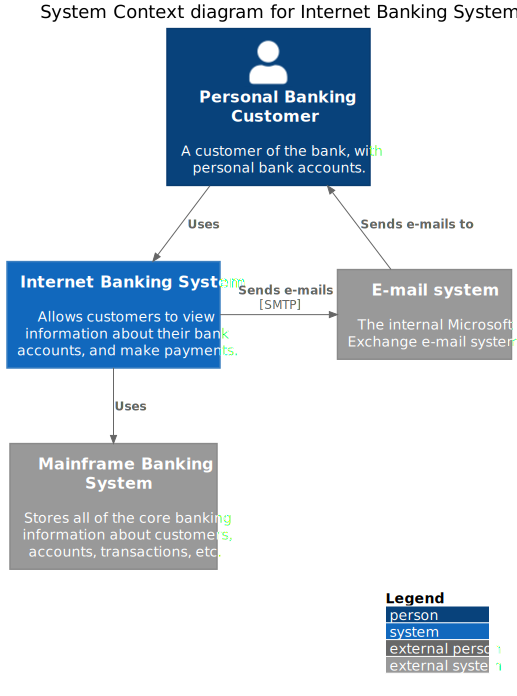
\includegraphics[height=15.00000cm]{generated/diagrams-examples-c4plantuml-context-Rmd.png}
\caption{Example - C4 Context Diagram}
\end{figure}

\begin{quote}
*NOTE: Диаграммы c4plantuml приходится скачивать в виде PNG для документов PDF, т.к. при переводе этих SVG в PDF не всё проходит корректно
\end{quote}

\newpage

\section{C4 Диаграмма контейнеров (PlantUML+C4)}\label{c4---plantumlc4}

Визуализатор: \texttt{c4plantuml}

\begin{figure}
\centering
\includegraphics[width=1.00000\textwidth]{generated/diagrams-examples-c4plantuml-container-Rmd.png}
\caption{Example - C4 Container Diagram}
\end{figure}

\begin{quote}
*NOTE: Диаграммы c4plantuml приходится скачивать в виде PNG для документов PDF, т.к. при переводе этих SVG в PDF не всё проходит корректно
\end{quote}

\newpage

\section{C4 Диаграмма компонентов (PlantUML+C4)}\label{c4---plantumlc4}

Визуализатор: \texttt{c4plantuml}

\begin{figure}
\centering
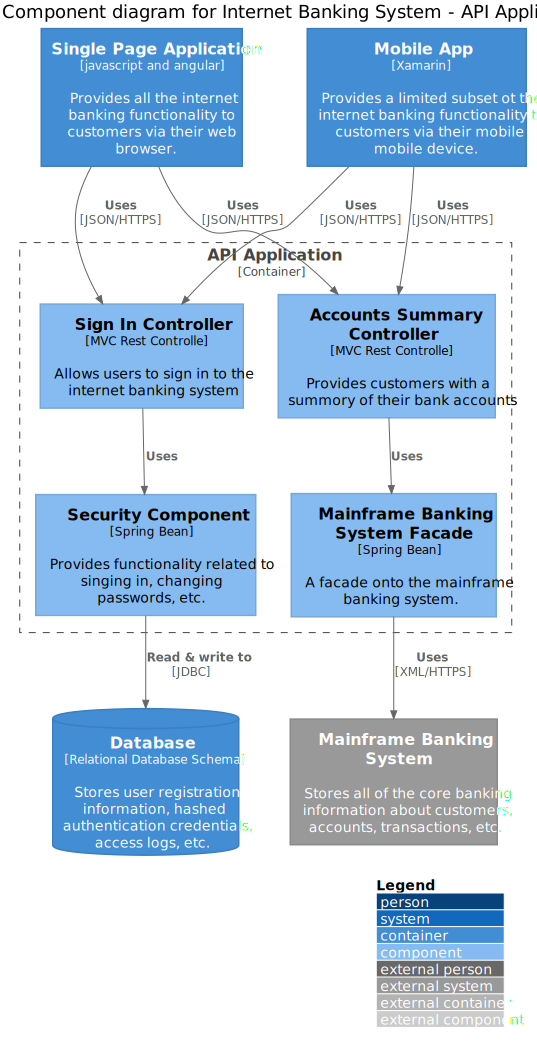
\includegraphics[height=15.00000cm]{generated/diagrams-examples-c4plantuml-component-Rmd.png}
\caption{Example - C4 Component Diagram}
\end{figure}

\begin{quote}
*NOTE: Диаграммы c4plantuml приходится скачивать в виде PNG для документов PDF, т.к. при переводе этих SVG в PDF не всё проходит корректно
\end{quote}

\newpage

\section{Блоксхема}

Визуализатор: \texttt{blockdiag}

\begin{figure}
\centering
\includegraphics{generated/diagrams-examples-blockdiag-Rmd.pdf}
\caption{Example - Block Diagram}
\end{figure}

\newpage

\section{Цифровая временная диаграмма}\label{--}

Визуализатор: \texttt{wavedrom}

\begin{figure}
\centering
\includegraphics{generated/diagrams-examples-wavedrom-Rmd.pdf}
\caption{Example - Digital Timing Diagram}
\end{figure}

\newpage

\section{Bytefield}\label{bytefield}

Визуализатор: \texttt{bytefield}

\begin{figure}
\centering
\includegraphics{generated/diagrams-examples-bytefield-Rmd.pdf}
\caption{Example - Bytefield}
\end{figure}

\newpage

\section{Packet Diagram}\label{packet-diagram}

Визуализатор: \texttt{packetdiag}

\begin{figure}
\centering
\includegraphics[width=1.00000\textwidth]{generated/diagrams-examples-packetdiag-Rmd.pdf}
\caption{Example - Packet Diagram}
\end{figure}

\newpage

\section{Диаграмма последовательности №1 (PlantUML)}\label{--1-plantuml}

Визуализатор: \texttt{plantuml}

\begin{figure}
\centering
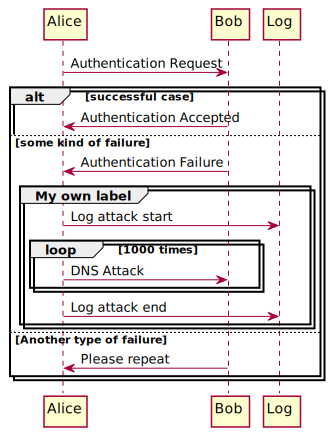
\includegraphics{generated/diagrams-examples-plantuml-seqdiag-Rmd.pdf}
\caption{Example - Sequence Diagram - PlantUML}
\end{figure}

\newpage

\section{Диаграмма последовательности №2 (SeqDiag)}\label{--2-seqdiag}

Визуализатор: \texttt{seqdiag}

\begin{figure}
\centering
\includegraphics{generated/diagrams-examples-seqdiag-Rmd.pdf}
\caption{Example - Sequence Diagram - SeqDiag}
\end{figure}

\newpage

\section{Граф фиксации изменений}\label{--}

Визуализатор: \texttt{pikchr}

\begin{quote}
\emph{NOTE: pikchr создаёт SVG, которые нормально отображают только Web-браузеры, поэтому с ними будут проблемы в PDF/PNG}
\end{quote}

\newpage

\section{Диаграмма прецедентов}\label{-}

Визуализатор: \texttt{plantuml}

\begin{figure}
\centering
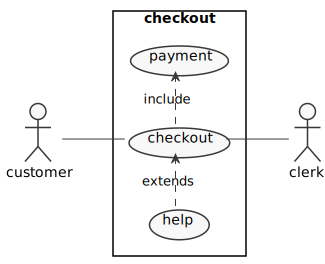
\includegraphics{generated/diagrams-examples-plantuml-usecase-Rmd.pdf}
\caption{Example Block Diagram}
\end{figure}

\newpage

\section{Ментальная карта}\label{-}

Визуализатор: \texttt{plantuml}

\begin{figure}
\centering
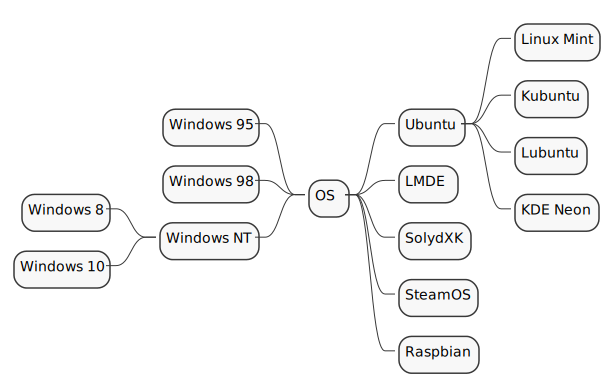
\includegraphics{generated/diagrams-examples-plantuml-mindmap-Rmd.pdf}
\caption{Example - Mind Map}
\end{figure}

\newpage

\section{PlantUML (ещё примеры)}\label{plantuml--}

В PlantUML возможно создание большого кол-ва диаграмм разного рода, таких как временные диаграммы, диаграмма Ганта и т.д..

Они все могут быть использованы аналогично предыдущим примерам.

Обратитесь к документации PlantUML \url{https://plantuml.com/} для подробностей их описания.

\newpage

\section{Диаграмма Ганта}\label{-}

Визуализатор: \texttt{mermaid}

\begin{quote}
\emph{NOTE: mermaid создаёт SVG, которые нормально отображают только Web-браузеры, поэтому с ними будут проблемы в PDF/PNG}
\end{quote}

\begin{figure}
\centering
\includegraphics{generated/diagrams-examples-mermaid-gantt-Rmd.pdf}
\caption{Example - Gantt}
\end{figure}

\bibliography{book.bib,packages.bib}

\end{document}
